\documentclass[11pt,a4paper]{article}
\usepackage[T1]{fontenc}
\usepackage[utf8]{inputenc}
\usepackage{lmodern,microtype}
\usepackage[a4paper,left=2.0cm,right=2.0cm,top=1.8cm,bottom=1.8cm]{geometry}
\usepackage{amsmath,amssymb,booktabs,array,tabularx,longtable}
\usepackage{xcolor,graphicx,float,enumitem,setspace}
\usepackage{titlesec,fancyhdr,lastpage}
\usepackage[hidelinks]{hyperref}
\usepackage{tikz}
\usetikzlibrary{positioning,arrows.meta,calc,fit,patterns,decorations.pathreplacing}

\definecolor{titleblue}{HTML}{005293}
\definecolor{waterblue}{HTML}{66B5D8}
\definecolor{coffeebrown}{HTML}{8B5A3C}
\definecolor{fineorange}{HTML}{E87722}
\definecolor{modelgreen}{HTML}{4C956C}
\definecolor{datagray}{HTML}{E8E8E8}
\definecolor{softcream}{HTML}{FFF5DF}

\setlength{\parindent}{0pt}
\setlength{\parskip}{0.55em}
\setlength{\emergencystretch}{2em}
\setstretch{1.04}
\setlist{itemsep=1.5pt,topsep=3pt,leftmargin=1.6em}
\titleformat{\section}{\large\bfseries\color{titleblue}}{\thesection}{0.6em}{}
\titleformat{\subsection}{\normalsize\bfseries\color{titleblue!85!black}}{\thesubsection}{0.6em}{}
\pagestyle{fancy}
\fancyhf{}
\lhead{\small FineFlow--Espresso}
\rhead{\small Technical documentation}
\cfoot{\small Page \thepage\ of \pageref{LastPage}}
\renewcommand{\headrulewidth}{0.3pt}

\newcommand{\pos}[1]{\left[#1\right]_+}
\newcommand{\dd}{\,\mathrm d}
\newcommand{\code}[1]{\texttt{#1}}
\graphicspath{{../results/}{../verification_results/}}

\begin{document}

\pagenumbering{gobble}
\begin{titlepage}
\centering
\vspace*{2.2cm}
{\Huge\bfseries\color{titleblue} FineFlow--Espresso\par}
\vspace{0.5cm}
{\LARGE A reduced one-dimensional model for fines release, migration,
blockage, detachment and cup washout\par}
\vspace{1.0cm}
{\Large Technical model and numerical documentation\par}
\vfill
{\large Ali Khalifa and Heiko Briesen\par}
\vspace{0.2cm}
{\normalsize Technical University of Munich\par
Chair of Process Systems Engineering\par}
\vfill
{\normalsize Demonstrator version documented from the current Python implementation\par}
\vspace{0.3cm}
{\small The parameter values shown here are illustrative and uncalibrated.\par}
\end{titlepage}

\pagenumbering{roman}
\tableofcontents
\newpage
\pagenumbering{arabic}

\section{Purpose and scope}

FineFlow--Espresso is a transparent continuum demonstrator for the coupled
hydraulics and transport of coffee fines through an espresso puck. The main
objective is to predict how initially attached fines are released, transported,
deposited, and possibly detached again; how these processes alter local
permeability; and how the changing resistance affects machine pressure and flow.
The model additionally distinguishes fines leaving the puck from fines retained
by the portafilter basket and fines entering the cup.

The model is deliberately one-dimensional. It is intended to organize
measurements, test mechanistic hypotheses, and provide interpretable predictions
without resolving each pore. It is not a substitute for pore-scale simulation.
Computed axial blockage locations are effective model states rather than direct
predictions of lateral channel geometry.

The software supports three levels of structural information:
\begin{enumerate}
  \item uniform initial porosity and permeability;
  \item depth-resolved initial profiles obtained from measurements or image analysis;
  \item a tabulated deposit--permeability relationship supplied by pore-network modelling.
\end{enumerate}

\section{Physical picture and system boundary}

Water enters at the top of a puck of length $L$ and cross-sectional area $A$.
The axial coordinate $z$ points from the inlet, $z=0$, to the basket,
$z=L$. Fines can move among three puck inventories: available fines attached to
the coffee matrix, mobile fines in the pore liquid, and deposited fines. At the
puck outlet the mobile-fines flux is divided between a basket-retained inventory
and a cup inventory.

\begin{figure}[H]
\centering
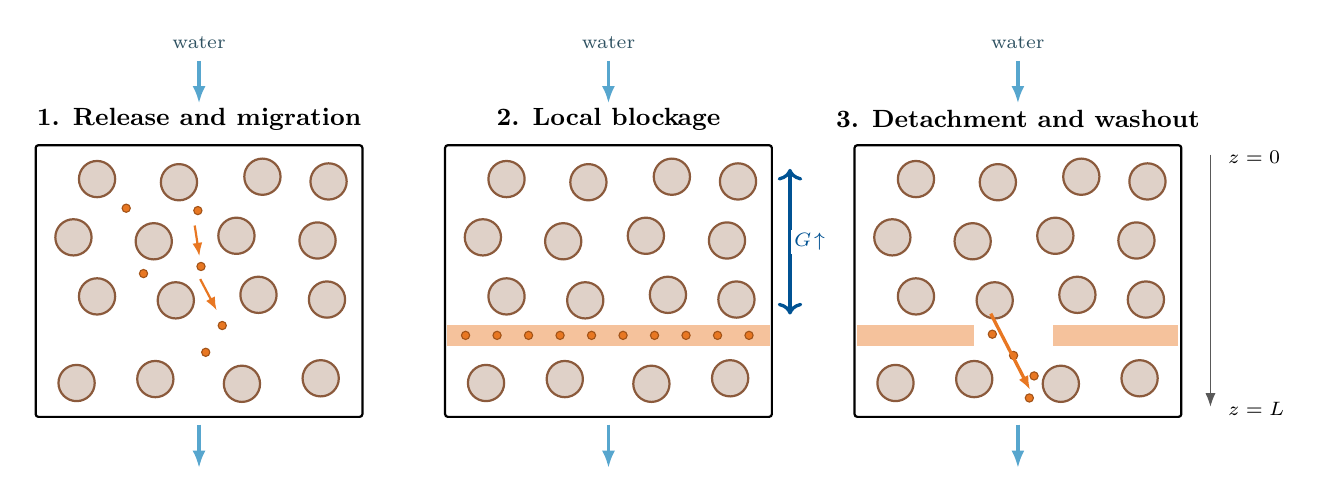
\begin{tikzpicture}[x=1cm,y=1cm,
 flow/.style={-{Latex[length=2.2mm]},very thick,waterblue!85!titleblue},
 fine/.style={circle,fill=fineorange,draw=fineorange!70!black,inner sep=1.05pt},
 grain/.style={circle,fill=coffeebrown!28,draw=coffeebrown,thick,minimum size=4.6mm},
 lab/.style={font=\small,align=center}]
\foreach \sx/\ttl in {0/{1. Release and migration},5.2/{2. Local blockage},10.4/{3. Detachment and washout}}{
  \begin{scope}[xshift=\sx cm]
    \draw[rounded corners=1pt,thick] (0,0) rectangle (4.15,3.45);
    \node[lab,font=\small\bfseries] at (2.075,3.78) {\ttl};
    \draw[flow] (2.075,4.52)--(2.075,3.98);
    \node[font=\scriptsize,text=waterblue!45!black] at (2.075,4.75) {water};
    \draw[flow] (2.075,-0.10)--(2.075,-0.65);
  \end{scope}
}
% Grains are deliberately separated from the fines pathways.
\foreach \sx in {0,5.2,10.4}{
 \foreach \x/\y in {.52/.43,1.52/.48,2.62/.42,3.62/.49,
                      .78/1.53,1.78/1.48,2.83/1.55,3.70/1.49,
                      .48/2.28,1.50/2.23,2.55/2.30,3.58/2.24,
                      .78/3.02,1.82/2.98,2.88/3.05,3.72/2.99}{
   \node[grain] at (\sx+\x,\y) {};
 }
}
% Panel 1: fines only in open voids.
\foreach \x/\y in {1.15/2.65,2.06/2.62,2.10/1.91,1.37/1.82,2.37/1.16,2.16/.82}
  \node[fine] at (\x,\y) {};
\draw[-{Latex[length=1.7mm]},fineorange,thick] (2.02,2.43)--(2.08,2.04);
\draw[-{Latex[length=1.7mm]},fineorange,thick] (2.09,1.75)--(2.30,1.35);
% Panel 2: thin effective deposit layer in an open inter-row gap.
\fill[fineorange!45] (5.23,.90) rectangle (9.32,1.17);
\foreach \x in {5.46,5.86,6.26,6.66,7.06,7.46,7.86,8.26,8.66,9.06}
  \node[fine] at (\x,1.035) {};
\draw[<->,very thick,titleblue] (9.58,1.30)--(9.58,3.15);
\node[font=\scriptsize\bfseries,titleblue,fill=white,inner sep=1.2pt]
  at (9.83,2.22) {$G\!\uparrow$};
% Panel 3: opening and downstream particles.
\fill[fineorange!45] (10.43,.90) rectangle (11.92,1.17);
\fill[fineorange!45] (12.92,.90) rectangle (14.51,1.17);
\foreach \x/\y in {12.15/1.05,12.42/.78,12.68/.52,12.62/.24}
  \node[fine] at (\x,\y) {};
\draw[-{Latex[length=1.8mm]},fineorange,very thick] (12.13,1.31)--(12.63,.34);
% Coordinate, placed outside all panels.
\draw[-{Latex[length=1.7mm]},black!65] (14.92,3.33)--(14.92,.13);
\node[font=\scriptsize,anchor=west] at (15.02,3.30) {$z=0$};
\node[font=\scriptsize,anchor=west] at (15.02,.10) {$z=L$};
\end{tikzpicture}
\caption{Effective one-dimensional mechanism. Mobile fines occupy open voids,
while an unresolved deposited layer is represented by a local mass inventory
and reduced effective permeability. If hydraulic loading exceeds an effective
strength, deposits detach. Only the fraction that can escape through the local
pore passages is returned to the mobile phase.}
\label{fig:mechanism}
\end{figure}

\subsection{Principal assumptions}

\begin{itemize}
  \item Water and suspended fines are incompressible, and the puck area is constant.
  \item The superficial velocity $q(t)=Q(t)/A$ is spatially uniform; local pore velocity is $q/\varepsilon$.
  \item Radial flow redistribution and explicit channels are not resolved.
  \item One effective fines population is used; particle-size-dependent transport is deferred.
  \item Fluid properties are constant and extraction chemistry, gas release, swelling, and thermal variation are omitted.
  \item Darcy--Forchheimer flow is evaluated as a one-dimensional algebraic
  pressure-gradient closure; no momentum PDE is solved.
  \item The basket model is level 1: constant hydraulic resistance and constant fines-retention fraction.
  \item Basket deposits do not yet modify basket resistance and cannot detach.
  \item Empirical closure parameters are effective quantities and require calibration.
\end{itemize}

\section{State variables and conservation laws}

The puck stores three fines inventories per unit bulk puck volume:
\begin{center}
\begin{tabularx}{0.92\textwidth}{@{}l l X@{}}
\toprule
Symbol & Unit & Meaning\\
\midrule
$m_{\mathrm a}(z,t)$ & kg m$^{-3}$ & available fines still attached to the coffee matrix\\
$\varepsilon c(z,t)$ & kg m$^{-3}$ & mobile fines per bulk volume; $c$ is per liquid volume\\
$m_{\mathrm d}(z,t)$ & kg m$^{-3}$ & deposited fines retained in the pore space\\
\bottomrule
\end{tabularx}
\end{center}

The continuum balances are
\begin{align}
 \frac{\partial(\varepsilon c)}{\partial t}
 +\frac{\partial(qc)}{\partial z}
 &=\frac{\partial}{\partial z}\!\left(\varepsilon D
 \frac{\partial c}{\partial z}\right)
 +R_{\mathrm{rel}}-R_{\mathrm{dep}}+R_{\mathrm{wash}}, \label{eq:mobile}\\
 \frac{\partial m_{\mathrm d}}{\partial t}
 &=R_{\mathrm{dep}}-R_{\mathrm{wash}}, \label{eq:deposit}\\
 \frac{\partial m_{\mathrm a}}{\partial t}
 &=-R_{\mathrm{rel}}. \label{eq:available}
\end{align}
Here $D$ is an effective axial dispersion coefficient. Integrating the three
equations over the puck shows that reaction terms cancel. Consequently, the
initial fines mass equals the sum of available, mobile, deposited, basket-retained,
and cup fines:
\begin{equation}
M_0=M_{\mathrm a}+M_{\mathrm m}+M_{\mathrm d}
 +M_{\mathrm{sieve}}+M_{\mathrm{cup}}. \label{eq:globalmass}
\end{equation}

\section{Constitutive and kinetic models}

\subsection{Release}

The available fines decay with a flow-dependent first-order rate:
\begin{align}
 R_{\mathrm{rel}}&=k_{\mathrm{rel}}m_{\mathrm a}f_q(q),\\
 f_q(q)&=\left(\frac{|q|}{q_{\mathrm{ref}}}\right)^{a_{\mathrm r}}.
\end{align}
The exact exponential fraction released over a numerical step $\Delta t$ is
$1-\exp[-k_{\mathrm{rel}}f_q\Delta t]$. This update is nonnegative and avoids
an additional reaction-stability restriction.

\subsection{Deposition}

The deposition closure is
\begin{equation}
 R_{\mathrm{dep}}=k_{\mathrm{dep}}\,\chi(z)\,|q|\,c
 \pos{1-\frac{m_{\mathrm d}}{m_{\mathrm{cap}}}}, \label{eq:deposition}
\end{equation}
where $k_{\mathrm{dep}}$ is a filtration coefficient, $m_{\mathrm{cap}}$ is
the local deposit capacity, and
\begin{equation}
\chi(z)=1+(\chi_{\mathrm out}-1)
\exp\!\left[-\frac{L-z}{\ell_{\mathrm out}}\right]
\end{equation}
is an optional empirical increase in capture near the basket. The latter is a
one-dimensional representation of stronger retention near the outlet and must
not be interpreted as resolved basket-hole geometry.

\subsection{Hydraulic detachment and geometric escape}

The revised model separates adhesion failure from successful remobilization.
Hydraulic loading first produces a potential detachment rate,
\begin{align}
R_{\mathrm{det}}^*&=k_{\mathrm{det}}m_{\mathrm d}
\pos{\frac{G}{G_{\mathrm{crit}}}-1}^{b},\\
G&=\left|\frac{\partial p}{\partial z}\right|.
\end{align}
The local hydraulic diameter is either supplied by CT/PNM or initialized from
the packed-bed surface relation
\begin{equation}
d_{\mathrm h,0}=\frac{2}{3}\,\phi_s d_{\mathrm{eff}}
\frac{\varepsilon_0}{1-\varepsilon_0}.
\end{equation}
With representative fine diameter $d_f$, the confinement ratio is
$\lambda=d_f/d_{\mathrm h}$. The net transfer to the mobile phase is
\begin{equation}
R_{\mathrm{wash}}=P_{\mathrm{esc}}(\lambda)R_{\mathrm{det}}^*.
\label{eq:washout}
\end{equation}
The default smooth closure is
\begin{equation}
P_{\mathrm{esc}}(\lambda)=
\frac{1}{1+\exp[s(\lambda-\lambda_c)]},
\end{equation}
where $\lambda_c$ is the 50\% escape ratio and $s$ controls transition
sharpness. Alternatively, the code accepts a PNM table of size ratio versus
escape probability. Potentially detached fines that do not escape are treated
as immediately recaptured locally. This avoids the discontinuity and weak
identifiability of a hard $d_f/d_h$ cutoff.

\subsection{Porosity and permeability}

Deposited fines reduce liquid-filled porosity according to
\begin{equation}
\varepsilon(z,t)=\max\!\left[\varepsilon_0(z)
-\frac{m_{\mathrm d}}{\rho_{\mathrm d}},\,\varepsilon_{\min}\right].
\end{equation}
The software provides three alternative permeability closures.

\paragraph{Exponential closure.}
\begin{equation}
\frac{K}{K_0}=\max\!\left[
\exp\!\left(-\beta\frac{m_{\mathrm d}}{m_{\mathrm{cap}}}\right),
\frac{K_{\min}}{K_0}\right]. \label{eq:kexp}
\end{equation}

\paragraph{Kozeny--Carman-style closure.}
\begin{equation}
\frac{K}{K_0}=
\left(\frac{\varepsilon}{\varepsilon_0}\right)^3
\left(\frac{1-\varepsilon_0}{1-\varepsilon}\right)^2,
\end{equation}
subject to the configured minimum ratio.

\paragraph{Pore-network table.}
For 
\code{permeability\_model = pnm\_table}, the code linearly interpolates a
user-provided table of $m_{\mathrm d}$ versus $K/K_0$. This allows a pore-network
calculation to define the continuum closure without forcing it into the
exponential form. Values outside the supplied deposit range use the nearest
table endpoint and are then bounded by the minimum permeability ratio.

\section{Hydraulics, machine control, and basket sieve}

\subsection{Darcy--Forchheimer puck resistance}

No momentum equation is solved. For constant area and incompressible flow, the
superficial velocity $q=Q/A$ is uniform in $z$, and the local pressure-gradient
magnitude is evaluated algebraically:
\begin{equation}
G(z,t)=\frac{\mu q}{K(z,t)}
 +\rho\beta_F(z,t)|q|q. \label{eq:df}
\end{equation}
The first term is viscous Darcy resistance. The second is nonlinear inertial
resistance, with Forchheimer coefficient $\beta_F$ in m$^{-1}$. Selecting
\code{hydraulic\_model = darcy} sets $\beta_F=0$. The optional evolution law
\begin{equation}
\beta_F=\beta_{F,0}\left(\frac{K_0}{K}\right)^{n_F}
\end{equation}
is available, but $n_F=0$ is recommended until PNM or experiments demonstrate
systematic evolution during blockage.

For positive flow, axial integration gives
\begin{equation}
\Delta p_{\mathrm{puck}}
=q\int_0^L\frac{\mu}{K}\dd z
q^2\int_0^L\rho\beta_F\dd z. \label{eq:dfintegrated}
\end{equation}
Consequently, prescribed-pressure operation requires only the positive root of
a scalar quadratic equation.

\subsection{Why Darcy--Forchheimer rather than direct Ergun}

Ergun estimates the complete resistance from porosity, sphericity and one
effective particle diameter. CT and the five-parameter PSD can supply these
quantities, but they do not retain connectivity, tortuosity, bottlenecks or
localized throat blockage. In Eq.~\eqref{eq:df}, $K(z,t)$ can instead be taken
directly from CT-based PNM or low-flow experiments, while $\beta_F$ represents
only the additional nonlinear resistance. The linear and quadratic parts can
be separated experimentally from $\Delta p=c_1Q+c_2Q^2$ using several imposed
flows. Ergun remains useful as a baseline and gives the estimate
\begin{equation}
\beta_{F,\mathrm{Ergun}}=
\frac{1.75(1-\varepsilon)}{\varepsilon^3d_{\mathrm{eff}}}.
\end{equation}
Thus Darcy--Forchheimer preserves resolved viscous structure while retaining
the inertial physics that motivates Ergun.

\subsection{Level-1 basket boundary}

The clean basket is a constant series resistance $R_{\mathrm s}$:
\begin{align}
\Delta p_{\mathrm{puck}}&=\displaystyle\int_0^LG\,\dd z,\\
\Delta p_{\mathrm{sieve}}&=Q R_{\mathrm s},\\
\Delta p_{\mathrm{total}}&=\Delta p_{\mathrm{puck}}+\Delta p_{\mathrm{sieve}}.
\label{eq:series}
\end{align}
If a fraction $\eta_{\mathrm s}$ of puck-outlet fines is retained, then
\begin{align}
\dot M_{\mathrm{cup}}&=(1-\eta_{\mathrm s})\dot M_{\mathrm{out,puck}},\\
\dot M_{\mathrm{sieve}}&=\eta_{\mathrm s}\dot M_{\mathrm{out,puck}}.
\end{align}
No sieve detachment term is present at level 1. Therefore, retention changes the
reported destination of fines but does not feed back into $R_{\mathrm s}$.

\subsection{Hydraulic operating modes}

\begin{description}[style=nextline,leftmargin=2.6cm]
\item[Flow mode] $Q(t)$ is prescribed and Eq.~\eqref{eq:series} predicts total pressure.
\item[Pressure mode] Total pressure is prescribed and the positive root of the
integrated Darcy--Forchheimer law gives $Q$. An optional pressure pulse can
challenge deposit stability.
\item[PI mode] The machine changes its flow command to approach a total-pressure target, subject to a pump-flow cap and actuator lag.
\end{description}

The PI implementation combines resistance-based feedforward with proportional
and integral correction. With pressure error $e=(p_{\mathrm{set}}-p)/10^5$ in bar,
\begin{align}
\Delta p(Q_{\mathrm{ff}})&=p_{\mathrm{set}},\\
Q_{\mathrm{raw}}&=Q_{\mathrm{ff}}+K_Pe+K_I\int e\dd t,\\
Q_{\mathrm{cmd}}&=\min\!\left[\max(Q_{\mathrm{raw}},0),Q_{\max}\right].
\end{align}
The actual flow approaches the command with first-order time constant $\tau_p$.
Conditional integration suppresses windup while the command is saturated. A
linear startup ramp can be applied to $p_{\mathrm{set}}$. Thus a sufficiently
permeable puck may stay below 9 bar when $Q_{\max}$ is reached.

\section{Initial and boundary conditions}

\subsection{Initial conditions}

Unless axial arrays are supplied, all cells begin with uniform
$\varepsilon_0$, $K_0$, $m_{\mathrm a,0}$, $m_{\mathrm d,0}$ and $c_0$.
Optional arrays 
\code{initial\_porosity\_profile} and
\code{initial\_permeability\_profile\_m2} must each contain exactly the number
of finite-volume cells. These arrays can represent depth-averaged results of CT
segmentation and pore-network flow calculations.

\subsection{Fines-transport boundaries}

At the water inlet, the incoming water contains no fines:
\begin{equation}
(qc)_{z=0}=0.
\end{equation}
The code imposes zero dispersive flux at both ends,
\begin{equation}
\left.\varepsilon D\frac{\partial c}{\partial z}\right|_{z=0,L}=0,
\end{equation}
and uses a convective outflow at $z=L$:
\begin{equation}
\dot M_{\mathrm{out,puck}}=Aq c(L,t).
\end{equation}
Reverse flow is not supported by the present demonstrator.

\subsection{Pressure boundaries}

The downstream cup is the zero-gauge-pressure reference. The pressure just
above the sieve is $\Delta p_{\mathrm{sieve}}$. The reconstructed puck pressure
therefore decreases from total inlet pressure to sieve pressure rather than to
zero. The remaining drop occurs across the lumped sieve resistance.

\section{Finite-volume discretization}

The interval $[0,L]$ is divided into $N$ control volumes of width
$\Delta z=L/N$. Cell-centred states are indexed by $i=1,\ldots,N$, while
advective and dispersive fluxes are evaluated at faces $i\pm\tfrac12$.

\begin{figure}[H]
\centering
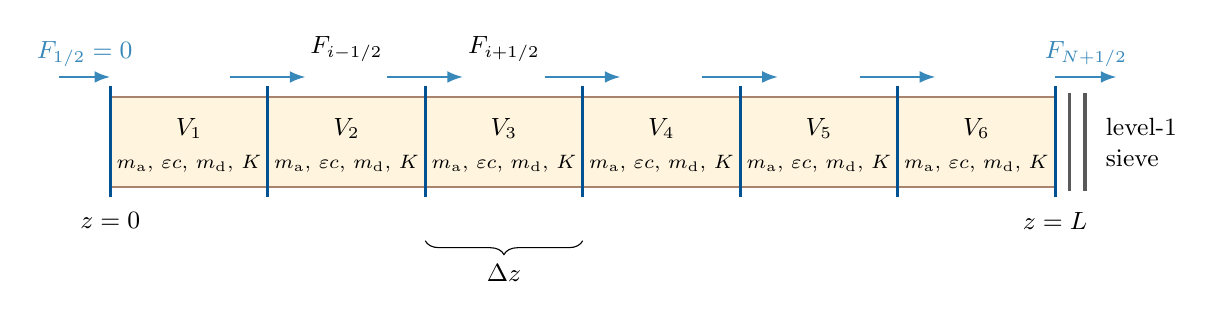
\begin{tikzpicture}[x=1cm,y=1cm,
 face/.style={very thick,titleblue},
 flux/.style={-{Latex[length=2mm]},thick,waterblue!55!titleblue},
 cell/.style={fill=softcream,draw=coffeebrown!75,thick},
 lab/.style={font=\small}]
\draw[flux] (-.65,1.40)--(0.0,1.40) node[midway,above,lab] {$F_{1/2}=0$};
\foreach \i [evaluate=\i as \x using 2*(\i-1)] in {1,...,6}{
  \draw[cell] (\x,0) rectangle ({\x+2},1.15);
  \node[lab] at ({\x+1},.75) {$V_{\i}$};
  \node[font=\scriptsize] at ({\x+1},.30) {$m_{\mathrm a},\,\varepsilon c,\,m_{\mathrm d},\,K$};
}
\foreach \x in {0,2,4,6,8,10,12}{\draw[face] (\x,-.13)--(\x,1.28);}
\foreach \x in {2,4,6,8,10}{\draw[flux] ({\x-.48},1.40)--({\x+.48},1.40);}
\draw[flux] (12,1.40)--(12.78,1.40) node[midway,above,lab] {$F_{N+1/2}$};
\node[lab,anchor=north] at (0,-.20) {$z=0$};
\node[lab,anchor=north] at (12,-.20) {$z=L$};
\draw[decorate,decoration={brace,mirror,amplitude=5pt}] (4,-.68)--(6,-.68)
 node[midway,below=5pt,lab] {$\Delta z$};
\node[lab] at (3,1.75) {$F_{i-1/2}$};
\node[lab] at (5,1.75) {$F_{i+1/2}$};
\draw[very thick,black!65] (12.18,-.05)--(12.18,1.20);
\draw[very thick,black!65] (12.38,-.05)--(12.38,1.20);
\node[lab,align=left,anchor=west] at (12.52,.57) {level-1\\sieve};
\end{tikzpicture}
\caption{One-dimensional finite-volume mesh. Reaction states are cell centred;
mobile-fines fluxes are face centred. The sieve is a lumped boundary element
after the last puck cell.}
\label{fig:fvm}
\end{figure}

Writing $u_i=(\varepsilon c)_i$, the mobile balance is discretized as
\begin{equation}
\frac{u_i^{n+1}-u_i^n}{\Delta t}
=-\frac{F_{i+1/2}-F_{i-1/2}}{\Delta z}
+R_{\mathrm{rel},i}-R_{\mathrm{dep},i}+R_{\mathrm{wash},i}.
\end{equation}
For forward flow, the face flux is
\begin{equation}
F_{i+1/2}=q c_i
-\varepsilon_{i+1/2}D\frac{c_{i+1}-c_i}{\Delta z}.
\end{equation}
Advection is first-order upwind and dispersion is centred. This combination is
conservative; the upwind part is monotone under the applied CFL restriction and
therefore does not create spurious oscillatory extrema in the pure-advection test.

The local Darcy--Forchheimer gradient is calculated in each cell. The discrete
puck pressure drop is
\begin{equation}
\Delta p_{\mathrm{puck}}=
\sum_{i=1}^{N}
\left(\frac{\mu q}{K_i}+\rho\beta_{F,i}|q|q\right)\Delta z.
\end{equation}
Face pressures are reconstructed by cumulative integration of the cell
gradients, starting from total inlet pressure and ending at sieve pressure.

\section{Time integration and solution algorithm}

The implementation uses explicit sequential operator splitting during each
time step:
\begin{enumerate}
  \item calculate porosity and permeability from the current deposit field;
  \item calculate Darcy--Forchheimer coefficients, flow, total pressure, local
  gradients and cell pressure;
  \item choose a stable time step;
  \item update release, deposition, potential detachment and size-selective
  escape with bounded exponential fractions;
  \item update mobile fines conservatively using face fluxes;
  \item split puck-outlet fines between basket and cup;
  \item update the PI controller and pump actuator when PI mode is active;
  \item record states at the requested output time.
\end{enumerate}

The time step is bounded by the user maximum, remaining time to the next output,
controller resolution, and a combined advection--dispersion estimate:
\begin{equation}
\Delta t\leq \frac{C_{\mathrm{CFL}}}
{|q|/(\varepsilon_{\min}\Delta z)+2D/\Delta z^2}.
\end{equation}
In PI mode, an additional limit $\Delta t\leq0.25\tau_p$ resolves the actuator.
Output times and pressure-pulse switching times are hit exactly.

\begin{figure}[H]
\centering
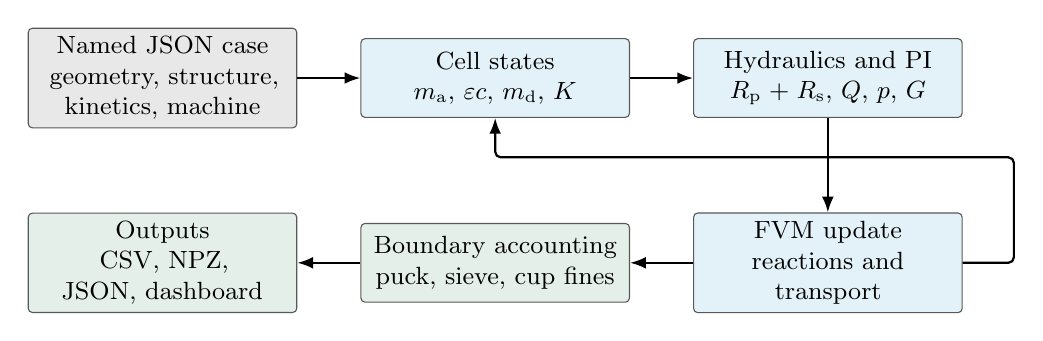
\begin{tikzpicture}[node distance=5mm and 8mm,
 box/.style={draw=black!65,rounded corners=1.5pt,minimum height=10mm,
 text width=3.2cm,align=center,font=\small,inner sep=3pt},
 data/.style={box,fill=datagray}, model/.style={box,fill=waterblue!18},
 resultbox/.style={box,fill=modelgreen!15}, arr/.style={-{Latex[length=2mm]},thick}]
\node[data] (inputs) {Named JSON case\\geometry, structure, kinetics, machine};
\node[model,right=of inputs] (state) {Cell states\\$m_{\mathrm a}$, $\varepsilon c$, $m_{\mathrm d}$, $K$};
\node[model,right=of state] (hyd) {Hydraulics and PI\\$R_{\mathrm p}+R_{\mathrm s}$, $Q$, $p$, $G$};
\node[model,below=12mm of hyd] (update) {FVM update\\reactions and transport};
\node[resultbox,left=of update] (basket) {Boundary accounting\\puck, sieve, cup fines};
\node[resultbox,left=of basket] (outputs) {Outputs\\CSV, NPZ, JSON, dashboard};
\draw[arr] (inputs)--(state); \draw[arr] (state)--(hyd);
\draw[arr] (hyd)--(update); \draw[arr] (update)--(basket);
\draw[arr] (basket)--(outputs);
\draw[arr,rounded corners=2pt]
(update.east) -- ++(.65,0)
|- ([yshift=-5mm]state.south)
-- (state.south);
\end{tikzpicture}
\caption{Computational workflow for one named case.}
\label{fig:workflow}
\end{figure}

\section{Configuration and calibration strategy}

Each named JSON case is applied on top of the Python defaults. A selected case
does not inherit values from another JSON case. Command-line options override
both defaults and the selected case. Generated parameter JSON files contain the
complete parameter set actually used.

For reproducible calibration, parameters are divided by the information source
that can actually identify them.

\begin{longtable}{@{}>{\raggedright\arraybackslash}p{2.7cm}
>{\raggedright\arraybackslash}p{4.4cm}
>{\raggedright\arraybackslash}p{7.2cm}@{}}
\toprule
Category & Parameters or fields & Determination method\\
\midrule
\endfirsthead
\toprule
Category & Parameters or fields & Determination method\\
\midrule
\endhead
Measured and fixed &
$L$, $A$, $\mu$, $\rho$, dose, PSD, $d_f$, $d_{\mathrm{eff}}$ &
Direct geometry and temperature measurements. Fit the Bora--Briesen
five-parameter bimodal volume PSD; calculate the fraction below a selected
mobility cutoff and conditional fine/coarse diameters. The PSD parameters are
inputs, not kinetic fit parameters.\\
\addlinespace
CT-derived structure &
$\varepsilon_0(z)$, $d_{\mathrm h,0}(z)$, deposit location &
Segment connected void and solid in axial slabs. Calculate
$d_h=4V_{\mathrm{void}}/A_{\mathrm{wetted}}$ and quantify voxel and
segmentation uncertainty. Use replicated interrupted shots to observe
structural changes.\\
\addlinespace
PNM-derived closures &
$K_0(z)$, $K/K_0(m_d)$, $d_h/d_{h,0}(m_d)$, $D$, capture and
$P_{\mathrm{esc}}(d_f/d_h)$ &
Solve network flow and particle transport on CT-derived networks. Sample the
measured PSD, record deposition, breakthrough, conductance loss and escape,
then export lookup tables. Scale the global PNM resistance to an independent
bulk low-flow measurement if required.\\
\addlinespace
Hydraulic experiments &
global $K$ scale, $\beta_F(z)$, $R_s$ &
Measure $\Delta p(Q)$ at several imposed flows and fit
$\Delta p=c_1Q+c_2Q^2$. Low-flow data constrain $K$; a broad flow range is
needed for $\beta_F$. Determine clean-basket resistance separately.\\
\addlinespace
Machine characterization &
$Q_{\max}$, $\tau_p$, pressure target, PI gains &
Measure pressure and flow without coffee and with known resistances. Fix these
before fitting puck kinetics.\\
\addlinespace
Dynamic fines experiments &
releasable inventory, $k_{\mathrm{rel}}$, $k_{\mathrm{det}}$,
$G_{\mathrm{crit}}$, $\eta_s$ &
Use time-resolved cup-fines mass or turbidity, preferably outlet PSD, together
with pressure and flow. Pressure pulses help separate threshold and rate.
Measure basket-retained mass independently where possible.\\
\bottomrule
\end{longtable}

The recommended sequence is: (1) fix geometry, fluid properties, dose and PSD;
(2) insert CT porosity and hydraulic-diameter profiles; (3) determine $K$ and
$\beta_F$ from pressure--flow experiments; (4) import PNM blockage, dispersion
and escape tables; (5) characterize basket and machine; (6) fit release to
early fines washout; and (7) fit detachment to controlled pressure events.
Validation must use withheld pucks or grind settings.

A single static CT image cannot determine release or detachment kinetics. Nor
can pressure and flow alone separate release, deposition, permeability loss,
detachment and basket capture. Fitting all parameters simultaneously would
therefore be structurally non-identifiable.

\section{Generated demonstration results}

Figure~\ref{fig:dashboard} is generated directly by the current Python solver
for the selected illustrative 
\code{fine\_puck} case. It shows the PI-controlled hydraulic response, the
distinction between puck-outlet and cup fines, and the evolving deposit and
relative-permeability fields.

\begin{figure}[H]
\centering
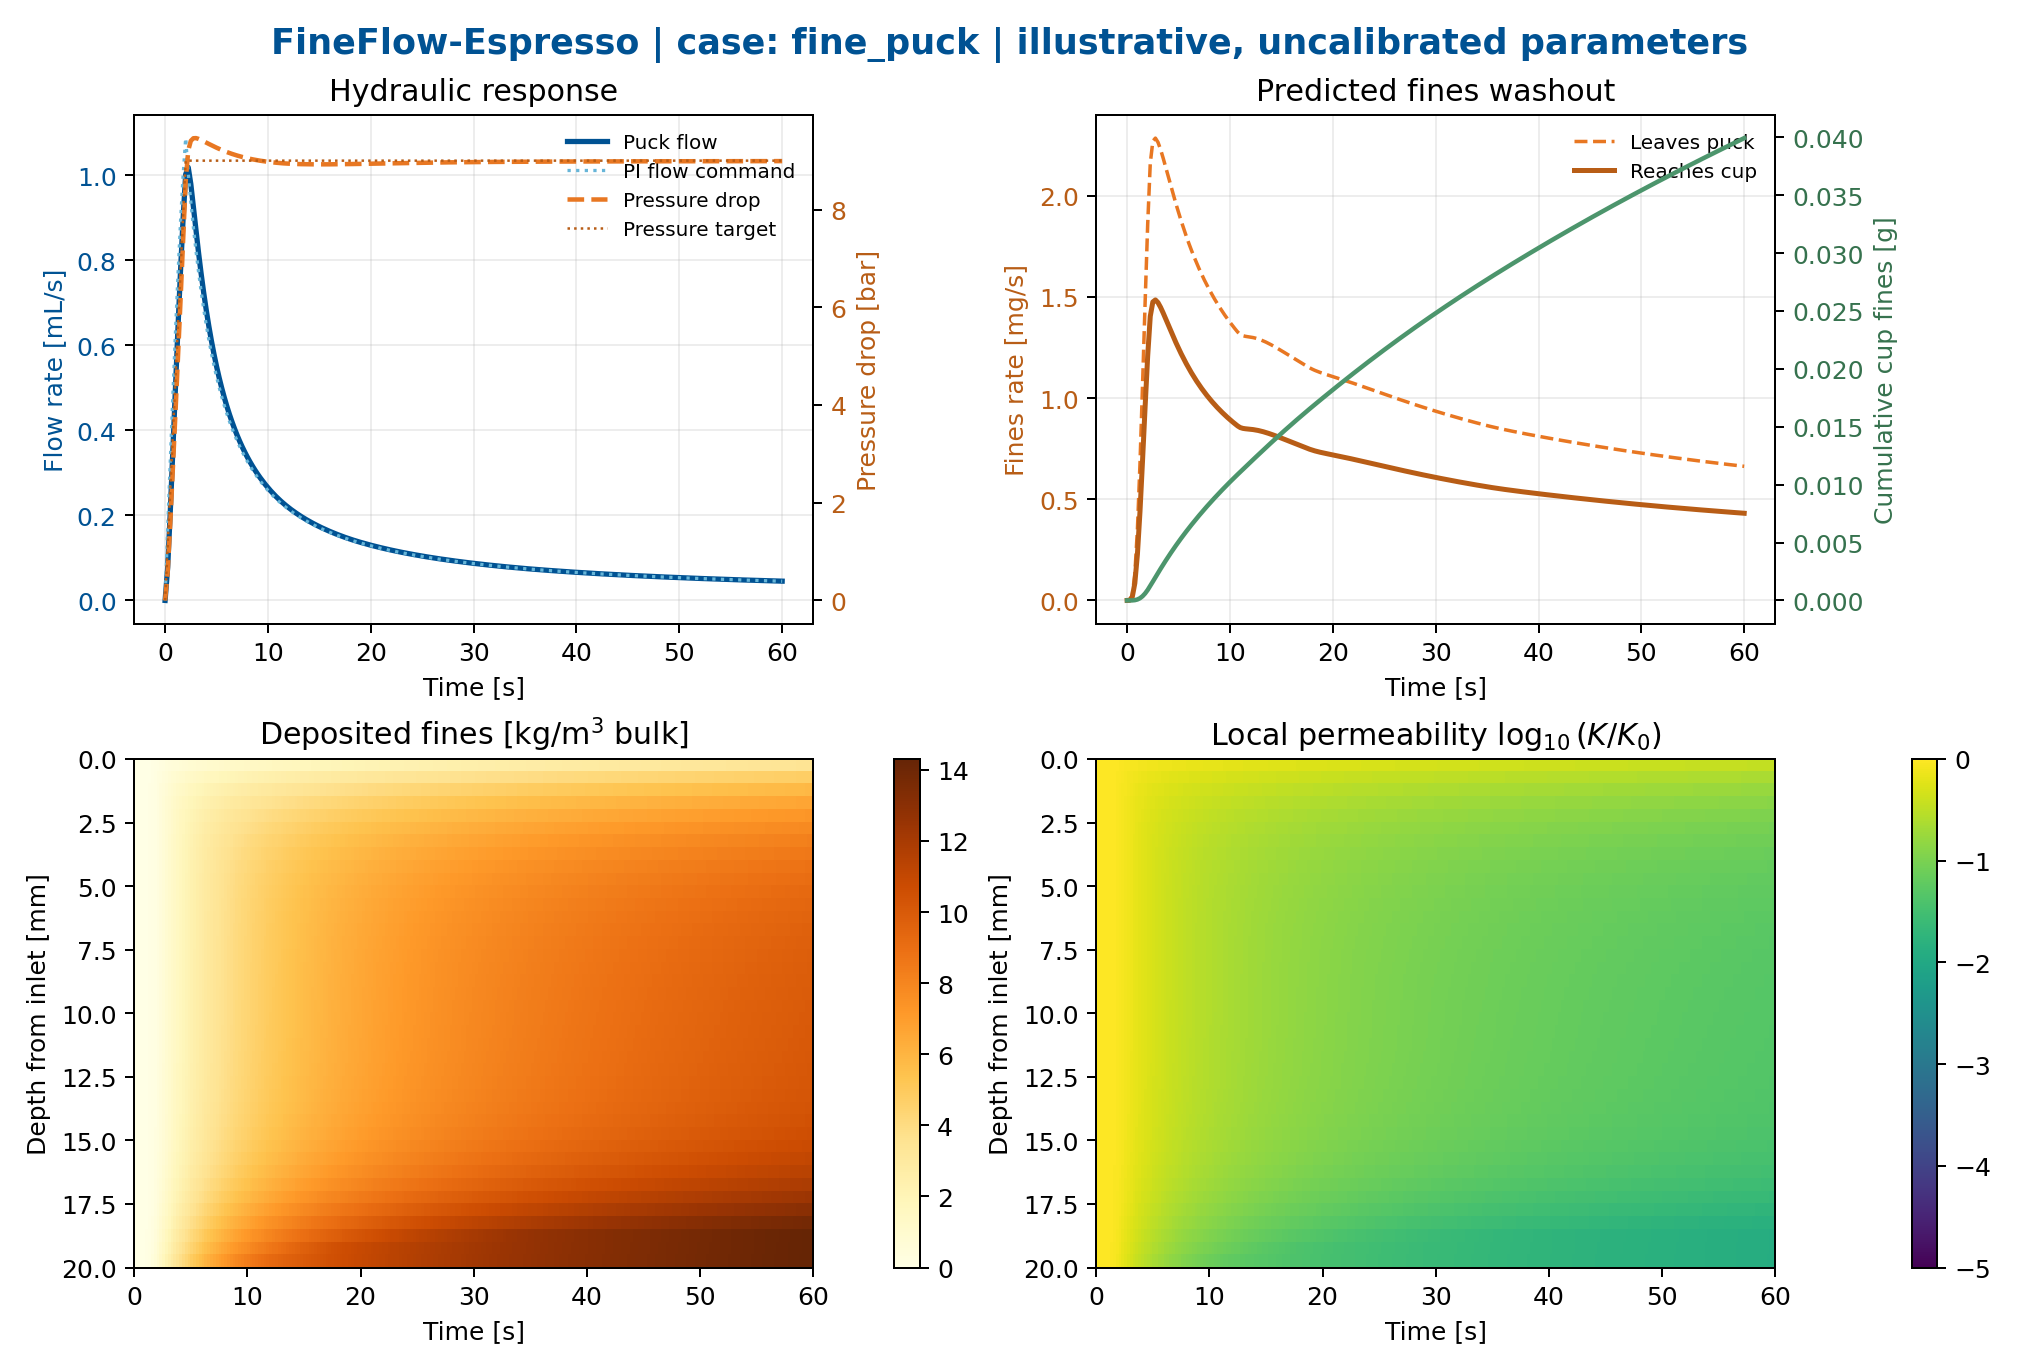
\includegraphics[width=0.98\textwidth]{fine_puck_dashboard.png}
\caption{Current illustrative fine-puck result. Parameters are not calibrated.}
\label{fig:dashboard}
\end{figure}

Selected final quantities are listed in Table~\ref{tab:result}. The basket
retains 35\% of the fines crossing the puck boundary by construction. The
sieve pressure contribution is small at the final low flow because the level-1
resistance is constant.

\begin{table}[H]
\centering
\caption{Illustrative result generated by the current code.}
\label{tab:result}
\begin{tabular}{@{}lr@{}}
\toprule
Quantity & Value\\
\midrule
Final total pressure drop & 8.9906 bar\\
Final puck pressure drop & 8.9902 bar\\
Final Forchheimer contribution & $5.88\times10^{-9}$ bar\\
Final sieve pressure drop & 0.00045 bar\\
Final flow rate & 0.0453 mL s$^{-1}$\\
Fines leaving puck & 0.06143 g\\
Fines retained by basket & 0.02150 g\\
Fines reaching cup & 0.03993 g\\
Minimum local $K/K_0$ & 0.01263\\
Minimum final hydraulic diameter & 76.58 $\mu$m\\
Maximum final $d_f/d_h$ & 0.3264\\
Mean final escape probability & 0.6447\\
Maximum relative mass error & $1.32\times10^{-15}$\\
\bottomrule
\end{tabular}
\end{table}

For the illustrative fine-puck parameters, the Forchheimer contribution is
negligible because the calibrated-looking permeability value produces a strongly
viscous-dominated resistance at the predicted flow. This is a model result, not
a reason to remove the term: coarse high-flow cases can show a larger
contribution, and the measured $\Delta p(Q)$ curvature must determine
$\beta_F$.

\section{Numerical verification}

Verification asks whether the equations are solved correctly; validation asks
whether those equations and calibrated parameters represent real espresso.
The repository contains conventional unit tests and an extended verification
program. The present version passes 15 unit tests and 17 extended checks.

The extended suite includes:
\begin{itemize}
  \item comparison with exact uniform-bed Darcy and Darcy--Forchheimer pressure;
  \item exact nonlinear inversion under prescribed pressure;
  \item superficial-velocity continuity and finite pore velocity;
  \item global fines conservation, positivity, porosity and permeability bounds;
  \item comparison of the release-only model with its analytical exponential solution;
  \item suppression of successful washout as $d_f/d_h$ increases;
  \item total-variation-diminishing and positivity checks for pure advection;
  \item spatial and temporal refinement studies;
  \item attainable PI target, pump-cap enforcement, and coarse-bed saturation behaviour.
\end{itemize}

\begin{figure}[H]
\centering
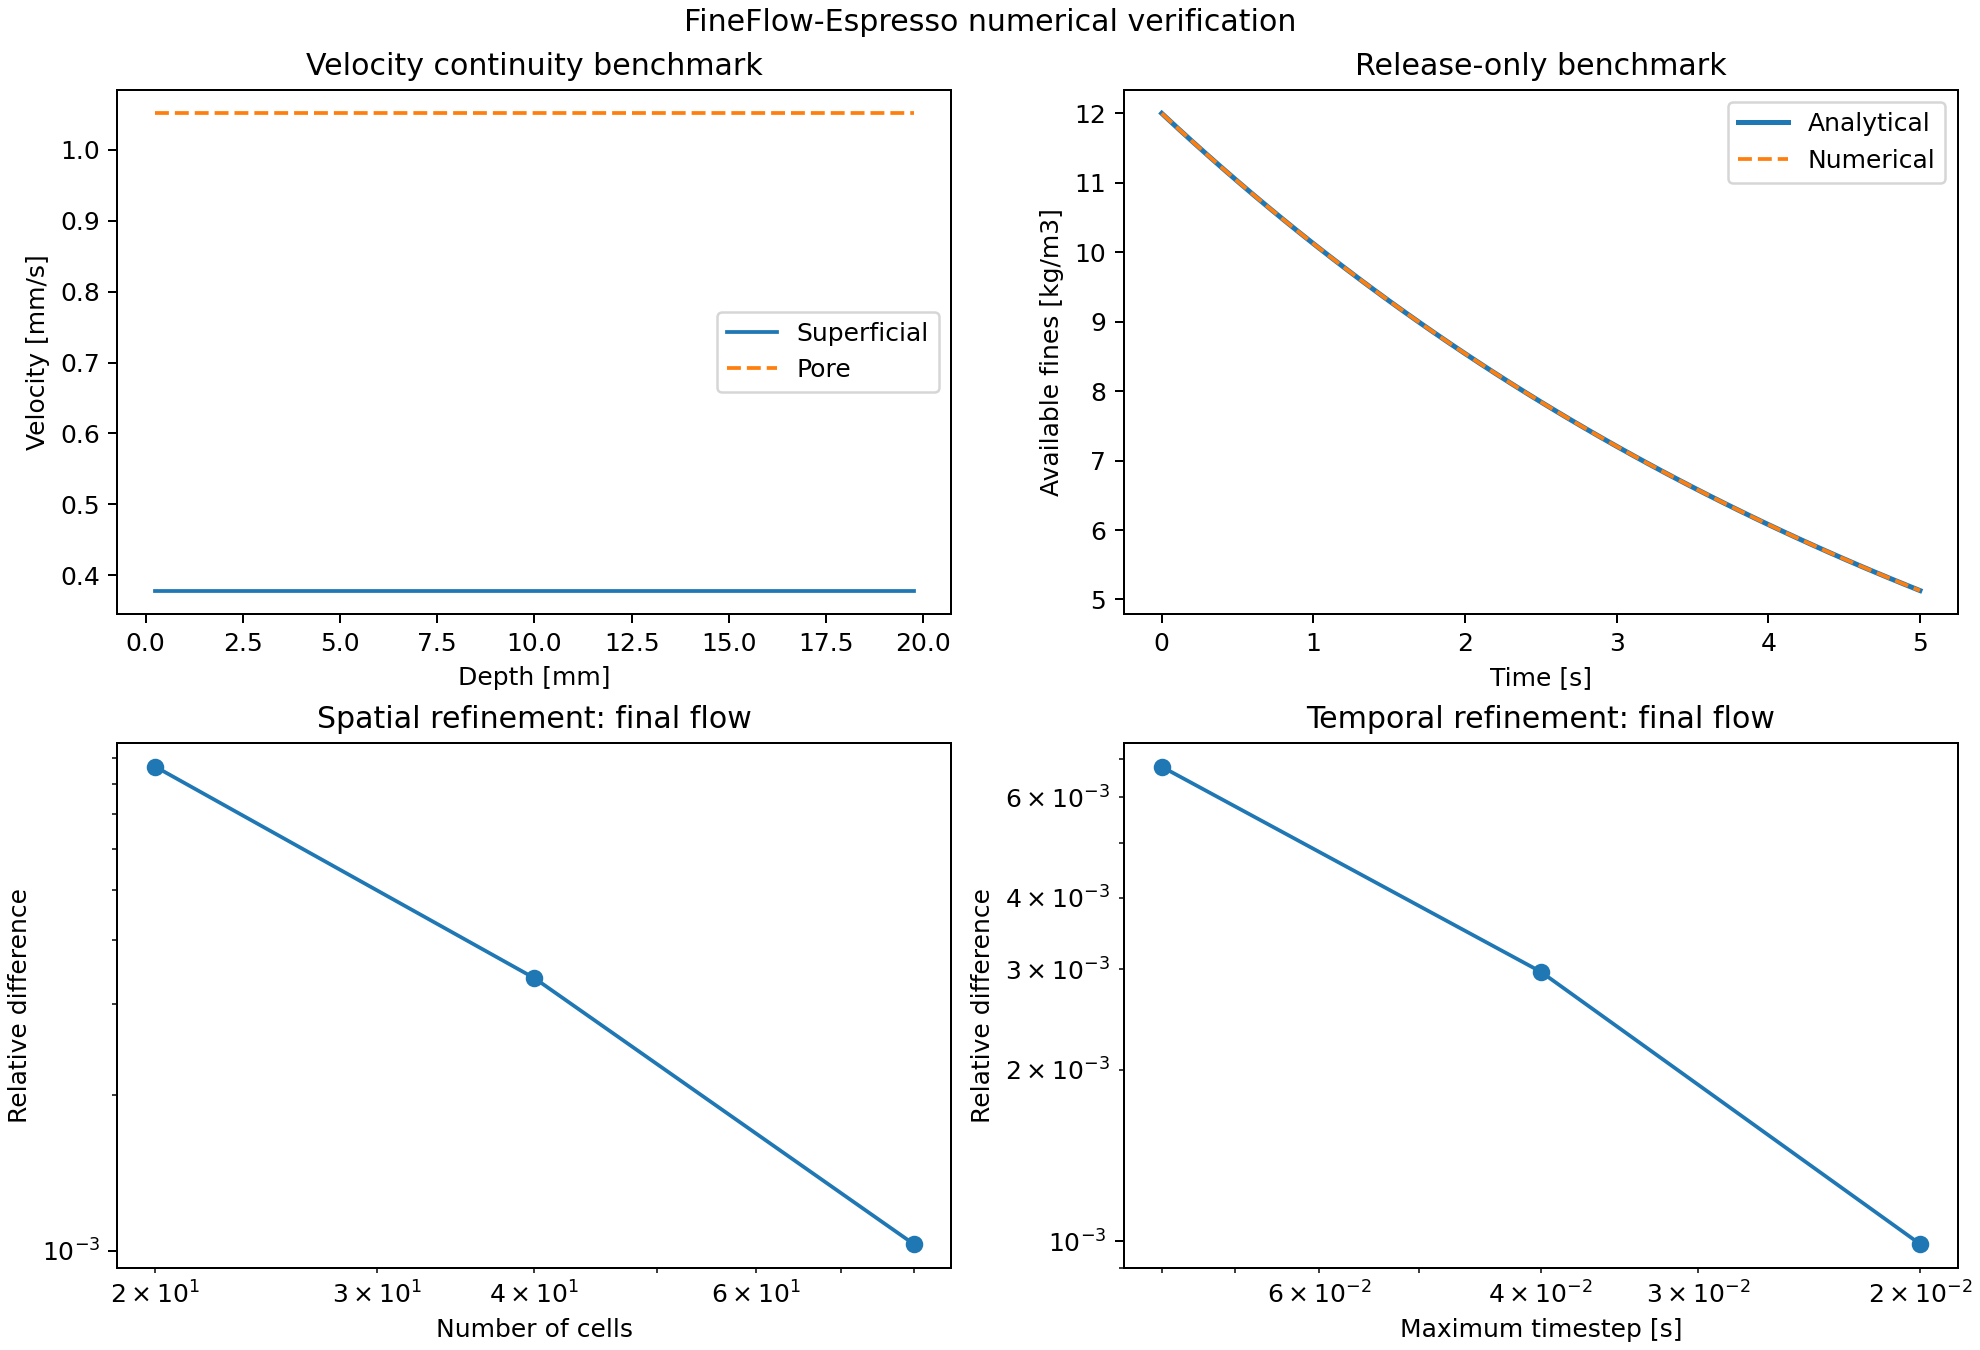
\includegraphics[width=0.98\textwidth]{verification_plots.png}
\caption{Automatically generated analytical and refinement diagnostics.}
\label{fig:verification}
\end{figure}

At the current settings, the maximum penultimate-to-finest difference across
the monitored quantities is approximately 2.9\% for spatial refinement and
0.45\% for temporal refinement. These are useful software checks, but they do
not establish model-form accuracy. Future verification should add a manufactured
solution for the complete coupled PDE system and formal observed-order estimates.

\section{Outputs and reproducibility}

For case name 
\code{fine\_puck}, the program writes:
\begin{itemize}
  \item 
  \code{fine\_puck\_timeseries.csv}: flow, controller command, pressure split,
  fines rates and cumulative destinations, blockage metrics, and mass error;
  \item 
  \code{fine\_puck\_profiles.npz}: time-dependent axial states, pressures,
  superficial and pore velocity, pressure gradient, Forchheimer coefficient,
  hydraulic diameter, size ratio, and escape probability;
  \item 
  \code{fine\_puck\_summary.json}: compact performance and conservation metrics;
  \item 
  \code{fine\_puck\_parameters.json}: complete parameters actually used;
  \item 
  \code{fine\_puck\_dashboard.png}: the four-panel result figure;
  \item four standalone manuscript panels for hydraulic response, fines
  washout, deposited fines and relative permeability, each as 600-dpi PNG and
  vector PDF.
\end{itemize}

The verification program writes a text report, pass/fail CSV, spatial and
temporal convergence tables, summary JSON, and verification figure. A nonzero
program exit status indicates that at least one verification criterion failed.

\section{Known limitations and planned extensions}

\begin{itemize}
  \item One fines class cannot represent size-dependent pore capture and basket passage.
  \item Level-1 basket resistance does not increase with retained fines.
  \item Basket-retained fines cannot detach or enter the cup later.
  \item Deposit-capacity and outlet-capture profiles are empirical.
  \item Static CT constrains structure but not unique kinetic parameters.
  \item Radial heterogeneity, lateral channels, cracks and individual basket holes are unresolved.
  \item Extraction, dissolution, temperature, gas, swelling and mechanical compaction are absent.
  \item The simple constant pump-flow cap should ultimately be replaced by a measured pump curve.
  \item Uncertainty propagation and parameter-identifiability analysis are not yet implemented.
\end{itemize}

The recommended next physical extension is a small number of fines-size classes
with size-dependent capture and sieve retention. The recommended next inference
extension is a calibration driver that reads measured pressure, flow, cup-fines,
CT-derived profiles, and PNM tables while marking parameters as fixed, informed
by priors, or fitted.

\section{How to compile and update this report}

From the 
\code{documentation} directory, compile with
\begin{verbatim}
latexmk -pdf fineflow_espresso_technical_report.tex
\end{verbatim}
The result and verification figures are referenced from the solver output
folders. Re-run the Python cases before recompiling when updated figures or
values are required. Numerical values in Table~\ref{tab:result} are currently
entered explicitly and should be updated when the reference case changes.

\end{document}
